\documentclass[11pt, a4paper]{article}

% Fonts and Encoding
\usepackage[utf8]{inputenc}
\usepackage[T1]{fontenc}
\usepackage{lmodern}


% Math and Symbols
\usepackage{amsmath, amssymb, amsthm, amsfonts, mathrsfs, mathtools}

% Layout and Geometry
\usepackage{geometry}
\geometry{a4paper, margin=1in}

% Formatting and Graphics
\usepackage{graphicx, xcolor, enumitem, booktabs, array, tabularx}

% TikZ for Illustrations
\usepackage{tikz}
\usetikzlibrary{arrows.meta, positioning, shapes.geometric, calc, backgrounds, matrix}

% Clickable Links and TOC
\usepackage{hyperref}
\hypersetup{
    colorlinks=true,
    linkcolor=blue,
    filecolor=magenta,      
    urlcolor=cyan,
    pdftitle={Advanced Mathematics: Relations and Properties},
}

% Theorem Environments
\newtheorem{theorem}{Theorem}[section]
\newtheorem{lemma}[theorem]{Lemma}
\newtheorem{proposition}[theorem]{Proposition}
\newtheorem{corollary}[theorem]{Corollary}
\theoremstyle{definition}
\newtheorem{definition}{Definition}[section]
\newtheorem{axiom}{Axiom}[section]
\newtheorem{example}{Example}[section]
\theoremstyle{remark}
\newtheorem{remark}{Remark}[section]

% Custom Commands (Enforced standard notation)
\newcommand{\R}{\mathbb{R}}
\newcommand{\N}{\mathbb{N}}
\newcommand{\Z}{\mathbb{Z}}
\newcommand{\Q}{\mathbb{Q}}
\newcommand{\E}{\mathbb{E}}
\newcommand{\Prob}{\mathbb{P}}
\newcommand{\F}{\mathcal{F}}
\newcommand{\dom}{\text{dom}}
\newcommand{\range}{\text{range}}

\title{\textbf{Advanced Abstract Mathematics: Relations and Their Properties}}
\author{Tashfeen Omran}
\date{\today}

\begin{document}

\maketitle
\tableofcontents
\newpage

% ==========================================
% PART 1: INTRODUCTION
% ==========================================
\section{Comprehensive Introduction, Context, and Prerequisites}

\subsection{Core Concepts \& Axioms}
At the heart of abstract mathematics lies the concept of a \textit{relation}, a formal structure that establishes associations between elements of sets. Before we can discuss functions, algebraic structures, or probability spaces, we must rigorously define how elements interact. 

\begin{definition}[Cartesian Product]
For any two sets $A$ and $B$, the Cartesian product $A \times B$ is the set of all ordered pairs $(a, b)$ where $a \in A$ and $b \in B$.
\[ A \times B = \{ (a, b) : a \in A \land b \in B \} \]
\end{definition}

\begin{definition}[Relation]
A relation $R$ from a set $A$ to a set $B$ is defined purely as a subset of the Cartesian product $A \times B$. If $(a, b) \in R$, we write $a \mathrel{R} b$. If $A = B$, we say $R$ is a relation \textit{on} $A$.
\end{definition}

\begin{definition}[Domain, Range, and Inverse]
For a relation $R \subseteq A \times B$:
\begin{itemize}
    \item \textbf{Domain:} $\dom(R) = \{ a \in A : \exists b \in B \text{ such that } (a, b) \in R \}$
    \item \textbf{Range:} $\range(R) = \{ b \in B : \exists a \in A \text{ such that } (a, b) \in R \}$
    \item \textbf{Inverse:} $R^{-1} = \{ (b, a) \in B \times A : (a, b) \in R \}$
\end{itemize}
\end{definition}

\subsection{Intuition and Set-Theoretic Foundations}
Intuitively, a relation is a rule of connectivity. If we visualize the elements of set $A$ as nodes on the left and elements of set $B$ as nodes on the right, a relation $R$ is simply a collection of directed arrows pointing from some nodes in $A$ to some nodes in $B$. 

When a relation is defined on a single set $A$ (i.e., $R \subseteq A \times A$), we can classify the "shape" of these connections using three foundational properties:
\begin{itemize}
    \item \textbf{Reflexivity:} Every node has a self-loop. ($\forall x \in A, x \mathrel{R} x$)
    \item \textbf{Symmetry:} Every one-way street is a two-way street. ($\forall x, y \in A, x \mathrel{R} y \implies y \mathrel{R} x$)
    \item \textbf{Transitivity:} If you can reach node $z$ from node $x$ via an intermediate node $y$, there is a direct express route from $x$ to $z$. ($\forall x, y, z \in A, (x \mathrel{R} y \land y \mathrel{R} z) \implies x \mathrel{R} z$)
\end{itemize}

\subsection{Historical Context and Motivation}
The formalization of relations emerged in the late 19th and early 20th centuries during the foundational crisis of mathematics. Mathematicians like Georg Cantor, Giuseppe Peano, and Felix Hausdorff sought to rebuild mathematics entirely upon set theory. Prior to this, concepts like "equality," "less than," and "functions" were treated as primitive, intuitive notions. By defining a relation strictly as a set of ordered pairs, mathematicians stripped away ambiguity, allowing for the rigorous development of equivalence classes, order theory, and topology.

\subsection{Prerequisites}
To master this chapter, the reader must possess:
\begin{enumerate}
    \item \textbf{Set Theory Fundamentals:} Understanding of subsets, intersections, unions, and power sets ($\mathcal{P}(A)$).
    \item \textbf{First-Order Logic:} Proficiency with universal ($\forall$) and existential ($\exists$) quantifiers, and logical implications ($\implies$).
    \item \textbf{Proof Techniques:} Mastery of direct proofs, proof by counterexample, and understanding \textit{vacuous truth} (a conditional statement is true if its antecedent is false).
\end{enumerate}

\newpage

% ==========================================
% PART 2: DETAILED HOMEWORK SOLUTIONS
% ==========================================
\section{Detailed Homework Solutions (Rigorous Proofs \& Computations)}

\subsection{Section 9.1 Exercises}

\textbf{Exercise 9.1.} For the sets $A = \{a, b, c\}$ and $B = \{r, s, t, u\}$, let $R = \{(a, s), (a, t), (b, t)\}$ be a relation from $A$ to $B$. Determine $\dom(R)$ and $\range(R)$.
\begin{proof}[Solution]
By definition, $\dom(R)$ is the set of all first coordinates of the ordered pairs in $R$, and $\range(R)$ is the set of all second coordinates.
\[ \dom(R) = \{ x \in A : \exists y \in B, (x, y) \in R \} = \{a, b\} \]
\[ \range(R) = \{ y \in B : \exists x \in A, (x, y) \in R \} = \{s, t\} \]
\end{proof}

\vspace{1em}
\textbf{Exercise 9.2.} Let $A$ be a nonempty set and let $B$ be a subset of the power set $\mathcal{P}(A)$ of $A$. Define a relation $R$ from $A$ to $B$ by $x \mathrel{R} Y$ if $x \in Y$. Give an example of two sets $A$ and $B$ that illustrate this. What is $R$ for these two sets?
\begin{proof}[Solution]
Let $A = \{1, 2, 3\}$. The power set $\mathcal{P}(A)$ contains all subsets of $A$. Let $B = \{\{1\}, \{1, 2\}, \{3\}\} \subseteq \mathcal{P}(A)$.
The relation $R$ consists of pairs $(x, Y)$ where $x \in A$, $Y \in B$, and $x \in Y$.
Checking each element of $A$ against each set in $B$:
\begin{itemize}
    \item For $Y = \{1\}$: $1 \in \{1\}$, so $(1, \{1\}) \in R$.
    \item For $Y = \{1, 2\}$: $1 \in \{1, 2\}$ and $2 \in \{1, 2\}$, so $(1, \{1, 2\}) \in R$ and $(2, \{1, 2\}) \in R$.
    \item For $Y = \{3\}$: $3 \in \{3\}$, so $(3, \{3\}) \in R$.
\end{itemize}
Thus, $R = \{ (1, \{1\}), (1, \{1, 2\}), (2, \{1, 2\}), (3, \{3\}) \}$.
\end{proof}

\vspace{1em}
\textbf{Exercise 9.3.} Let $A = \{0, 1\}$. Determine all the relations on $A$.
\begin{proof}[Solution]
A relation on $A$ is a subset of $A \times A$. First, we find $A \times A$:
\[ A \times A = \{ (0,0), (0,1), (1,0), (1,1) \} \]
Since $|A \times A| = 4$, there are $2^4 = 16$ possible subsets, and thus 16 relations on $A$. They are:
\begin{enumerate}[label=\arabic*., itemsep=0pt]
    \item $\emptyset$
    \item $\{(0,0)\}$
    \item $\{(0,1)\}$
    \item $\{(1,0)\}$
    \item $\{(1,1)\}$
    \item $\{(0,0), (0,1)\}$
    \item $\{(0,0), (1,0)\}$
    \item $\{(0,0), (1,1)\}$
    \item $\{(0,1), (1,0)\}$
    \item $\{(0,1), (1,1)\}$
    \item $\{(1,0), (1,1)\}$
    \item $\{(0,0), (0,1), (1,0)\}$
    \item $\{(0,0), (0,1), (1,1)\}$
    \item $\{(0,0), (1,0), (1,1)\}$
    \item $\{(0,1), (1,0), (1,1)\}$
    \item $\{(0,0), (0,1), (1,0), (1,1)\} = A \times A$
\end{enumerate}
\end{proof}

\vspace{1em}
\textbf{Exercise 9.4.} Let $A = \{a, b, c\}$ and $B = \{1, 2, 3, 4\}$. Then $R_1 = \{(a, 2), (a, 3), (b, 1), (b, 3), (c, 4)\}$ is a relation from $A$ to $B$, while $R_2 = \{(1, b), (1, c), (2, a), (2, b), (3, c), (4, a), (4, c)\}$ is a relation from $B$ to $A$. A relation $R$ is defined on $A$ by $x \mathrel{R} y$ if there exists $z \in B$ such that $x \mathrel{R_1} z$ and $z \mathrel{R_2} y$. Express $R$ by listing its elements.
\begin{proof}[Solution]
We must find all pairs $(x, y) \in A \times A$ connected via an intermediate element $z \in B$. We systematically check each pair in $R_1$:
\begin{itemize}
    \item $(a, 2) \in R_1$. In $R_2$, we have $(2, a)$ and $(2, b)$. This yields $(a, a) \in R$ and $(a, b) \in R$.
    \item $(a, 3) \in R_1$. In $R_2$, we have $(3, c)$. This yields $(a, c) \in R$.
    \item $(b, 1) \in R_1$. In $R_2$, we have $(1, b)$ and $(1, c)$. This yields $(b, b) \in R$ and $(b, c) \in R$.
    \item $(b, 3) \in R_1$. In $R_2$, we have $(3, c)$. This yields $(b, c) \in R$ (already listed).
    \item $(c, 4) \in R_1$. In $R_2$, we have $(4, a)$ and $(4, c)$. This yields $(c, a) \in R$ and $(c, c) \in R$.
\end{itemize}
Collecting all generated pairs, we obtain:
\[ R = \{ (a, a), (a, b), (a, c), (b, b), (b, c), (c, a), (c, c) \} \]
\end{proof}

\vspace{1em}
\textbf{Exercise 9.5.} For the relation $R = \{(1, 1), (1, 2), (1, 3), (2, 2), (2, 3), (3, 3)\}$ defined on the set $\{1, 2, 3\}$, what is $R^{-1}$?
\begin{proof}[Solution]
The inverse relation $R^{-1}$ is formed by reversing the coordinates of every ordered pair in $R$.
\[ R^{-1} = \{ (1, 1), (2, 1), (3, 1), (2, 2), (3, 2), (3, 3) \} \]
\end{proof}

\vspace{1em}
\textbf{Exercise 9.6.} A relation $R$ is defined on $\N$ by $a \mathrel{R} b$ if $a/b \in \N$. For $c, d \in \N$, under what conditions is $c \mathrel{R^{-1}} d$?
\begin{proof}[Solution]
By the definition of an inverse relation, $c \mathrel{R^{-1}} d$ if and only if $d \mathrel{R} c$. 
Applying the definition of $R$, $d \mathrel{R} c$ means that $d/c \in \N$. 
Since $c, d \in \N$, the statement $d/c \in \N$ is equivalent to saying that $c$ divides $d$ evenly (i.e., $c \mid d$). 
Therefore, $c \mathrel{R^{-1}} d$ under the condition that $c$ is a divisor of $d$.
\end{proof}

\vspace{1em}
\textbf{Exercise 9.7.} Determine the inverse relation $R^{-1}$ for the relation $R = \{(x, y) : x + 4y \text{ is odd}\}$ defined on $\N$.
\begin{proof}[Solution]
By definition, $R^{-1} = \{ (y, x) : (x, y) \in R \}$. 
Substituting the condition for $R$, we get:
\[ R^{-1} = \{ (y, x) \in \N \times \N : x + 4y \text{ is odd} \} \]
To express this in standard $(x, y)$ notation (where $x$ is the first coordinate and $y$ is the second), we swap the variable names:
\[ R^{-1} = \{ (x, y) \in \N \times \N : y + 4x \text{ is odd} \} \]
\end{proof}

\vspace{1em}
\textbf{Exercise 9.8.} For the relation $R = \{(x, y) : x \le y\}$ defined on $\N$, what is $R^{-1}$?
\begin{proof}[Solution]
By definition, $R^{-1} = \{ (y, x) : x \le y \}$. 
Swapping the variable names to maintain standard $(x, y)$ notation, we obtain:
\[ R^{-1} = \{ (x, y) \in \N \times \N : y \le x \} = \{ (x, y) \in \N \times \N : x \ge y \} \]
\end{proof}

\vspace{1em}
\textbf{Exercise 9.9.} Let $A$ and $B$ be sets with $|A| = |B| = 4$.
(a) Prove or disprove: If $R$ is a relation from $A$ to $B$ where $|R| = 9$ and $R = R^{-1}$, then $A = B$.
(b) Show that by making a small change in the statement in (a), a different response to the resulting statement can be obtained.
\begin{proof}[Solution]
\textbf{Part (a):} We will disprove the statement by providing a counterexample. 
Let $A = \{1, 2, 3, 4\}$ and $B = \{1, 2, 3, 5\}$. Clearly, $|A| = |B| = 4$ and $A \neq B$.
Let $R = \{1, 2, 3\} \times \{1, 2, 3\}$. 
Since $\{1, 2, 3\} \subseteq A$ and $\{1, 2, 3\} \subseteq B$, it follows that $R \subseteq A \times B$, making $R$ a valid relation from $A$ to $B$.
The number of elements in $R$ is $3 \times 3 = 9$.
Furthermore, $R^{-1} = \{ (y, x) : (x, y) \in \{1, 2, 3\} \times \{1, 2, 3\} \} = \{1, 2, 3\} \times \{1, 2, 3\} = R$.
Thus, all hypotheses are satisfied, but $A \neq B$. The statement is false.

\textbf{Part (b):} Change the condition $|R| = 9$ to $|R| = 10$. 
If $R = R^{-1}$, then $R \subseteq A \times B$ and $R \subseteq B \times A$. This implies $R \subseteq (A \times B) \cap (B \times A) = (A \cap B) \times (A \cap B)$.
Let $k = |A \cap B|$. The maximum number of elements in $(A \cap B) \times (A \cap B)$ is $k^2$.
If $|R| = 10$, then we must have $10 \le k^2$, which implies $k \ge 4$ (since $k$ is an integer).
Since $A$ and $B$ only have 4 elements, $k$ cannot exceed 4. Thus $k = 4$.
If $|A \cap B| = 4$ and $|A| = |B| = 4$, it strictly follows that $A = B$. The modified statement is true.
\end{proof}

\vspace{1em}
\textbf{Exercise 9.10.} Let $A$ be a set with $|A| = 4$. What is the maximum number of elements that a relation $R$ on $A$ can contain so that $R \cap R^{-1} = \emptyset$?
\begin{proof}[Solution]
The condition $R \cap R^{-1} = \emptyset$ means that if $(x, y) \in R$, then $(y, x) \notin R$.
First, this implies that for any $x \in A$, $(x, x) \notin R$ (otherwise $(x, x) \in R \cap R^{-1}$).
Second, for any pair of distinct elements $x, y \in A$ (where $x \neq y$), the relation $R$ can contain at most one of the ordered pairs $(x, y)$ or $(y, x)$.
The total number of distinct pairs $(x, y)$ with $x \neq y$ in $A \times A$ is $4 \times 3 = 12$.
These 12 pairs can be grouped into 6 mutually exclusive sets of the form $\{(x, y), (y, x)\}$.
To maximize $|R|$ while satisfying the condition, we select exactly one ordered pair from each of the 6 sets.
Therefore, the maximum number of elements in $R$ is 6.
\end{proof}

\subsection{Section 9.2 Exercises}

\textbf{Exercise 9.11.} Let $A = \{a, b, c, d\}$ and let $R = \{(a, a), (a, b), (a, c), (a, d), (b, b), (b, c), (b, d), (c, c), (c, d), (d, d)\}$ be a relation on $A$. Which of the properties reflexive, symmetric and transitive does the relation $R$ possess? If $R$ does not possess one of these properties, explain why.
\begin{proof}[Solution]
\begin{itemize}
    \item \textbf{Reflexive:} Yes. For every $x \in A$, $(x, x) \in R$. Specifically, $(a, a), (b, b), (c, c), (d, d) \in R$.
    \item \textbf{Symmetric:} No. We have $(a, b) \in R$, but $(b, a) \notin R$.
    \item \textbf{Transitive:} Yes. For any $x, y, z \in A$, if $(x, y) \in R$ and $(y, z) \in R$, then $(x, z) \in R$. (This relation is isomorphic to the standard $\le$ relation on an ordered set of 4 elements).
\end{itemize}
\end{proof}

\vspace{1em}
\textbf{Exercise 9.12.} Let $S = \{a, b, c\}$. Then $R = \{(a, a), (a, b), (a, c)\}$ is a relation on $S$. Which of the properties reflexive, symmetric and transitive does the relation $R$ possess? Justify your answers.
\begin{proof}[Solution]
\begin{itemize}
    \item \textbf{Reflexive:} No. The elements $b, c \in S$, but $(b, b) \notin R$ and $(c, c) \notin R$.
    \item \textbf{Symmetric:} No. We have $(a, b) \in R$, but $(b, a) \notin R$.
    \item \textbf{Transitive:} Yes. We must check all pairs where $(x, y) \in R$ and $(y, z) \in R$. The only such chains occur when $y = a$. If $(x, a) \in R$, then $x$ must be $a$. So the only chain is $(a, a) \in R$ and $(a, z) \in R \implies (a, z) \in R$, which is trivially true for $z \in \{a, b, c\}$.
\end{itemize}
\end{proof}

\vspace{1em}
\textbf{Exercise 9.13.} Let $S = \{a, b, c\}$. Then $R = \{(a, b)\}$ is a relation on $S$. Which of the properties reflexive, symmetric and transitive does the relation $R$ possess?
\begin{proof}[Solution]
\begin{itemize}
    \item \textbf{Reflexive:} No. $(a, a) \notin R$.
    \item \textbf{Symmetric:} No. $(a, b) \in R$ but $(b, a) \notin R$.
    \item \textbf{Transitive:} Yes. The condition for transitivity is: $\forall x, y, z, (x \mathrel{R} y \land y \mathrel{R} z) \implies x \mathrel{R} z$. Since there is no $y$ such that both $(x, y) \in R$ and $(y, z) \in R$ exist, the premise is false. Thus, the implication is \textit{vacuously true}.
\end{itemize}
\end{proof}

\vspace{1em}
\textbf{Exercise 9.14.} Let $A = \{a, b, c, d\}$. Give an example (with justification) of a relation $R$ on $A$ that has none of the following properties: reflexive, symmetric, transitive.
\begin{proof}[Solution]
Let $R = \{(a, b), (b, c)\}$.
\begin{itemize}
    \item \textbf{Not Reflexive:} $(a, a) \notin R$.
    \item \textbf{Not Symmetric:} $(a, b) \in R$, but $(b, a) \notin R$.
    \item \textbf{Not Transitive:} $(a, b) \in R$ and $(b, c) \in R$, but $(a, c) \notin R$.
\end{itemize}
\end{proof}

\vspace{1em}
\textbf{Exercise 9.15.} A relation $R$ is defined on $\Z$ by $a \mathrel{R} b$ if $|a - b| \le 2$. Which of the properties reflexive, symmetric and transitive does the relation $R$ possess? If $R$ does not possess one of these properties, explain why.
\begin{proof}[Solution]
\begin{itemize}
    \item \textbf{Reflexive:} Yes. For any $a \in \Z$, $|a - a| = 0 \le 2$. Thus $a \mathrel{R} a$.
    \item \textbf{Symmetric:} Yes. For any $a, b \in \Z$, if $a \mathrel{R} b$, then $|a - b| \le 2$. Since $|a - b| = |b - a|$, we have $|b - a| \le 2$, so $b \mathrel{R} a$.
    \item \textbf{Transitive:} No. Let $a = 1, b = 3, c = 5$. We have $|1 - 3| = 2 \le 2$ (so $1 \mathrel{R} 3$) and $|3 - 5| = 2 \le 2$ (so $3 \mathrel{R} 5$). However, $|1 - 5| = 4 \not\le 2$, so $1 \not\mathrel{R} 5$.
\end{itemize}
\end{proof}

\vspace{1em}
\textbf{Exercise 9.16.} Let $A = \{a, b, c, d\}$. How many relations defined on $A$ are reflexive, symmetric and transitive and contain the ordered pairs $(a, b), (b, c), (c, d)$?
\begin{proof}[Solution]
A relation that is reflexive, symmetric, and transitive is an equivalence relation. Equivalence relations uniquely partition a set into disjoint equivalence classes.
Since $R$ contains $(a, b)$, $a$ and $b$ are in the same equivalence class.
Since $R$ contains $(b, c)$, $b$ and $c$ are in the same equivalence class.
Since $R$ contains $(c, d)$, $c$ and $d$ are in the same equivalence class.
By transitivity, all elements $a, b, c, d$ must belong to the exact same equivalence class. 
Therefore, there is only one partition of $A$: the set $A$ itself. 
This corresponds to exactly one equivalence relation: the universal relation $R = A \times A$.
Answer: 1.
\end{proof}

\vspace{1em}
\textbf{Exercise 9.17.} Let $R = \emptyset$ be the empty relation on a nonempty set $A$. Which of the properties reflexive, symmetric and transitive does $R$ possess?
\begin{proof}[Solution]
\begin{itemize}
    \item \textbf{Reflexive:} No. Since $A$ is nonempty, there exists some $x \in A$. For $R$ to be reflexive, we must have $(x, x) \in R$. But $R = \emptyset$, so $(x, x) \notin R$.
    \item \textbf{Symmetric:} Yes (vacuously). The condition $(x, y) \in R \implies (y, x) \in R$ is vacuously true because the premise $(x, y) \in R$ is always false.
    \item \textbf{Transitive:} Yes (vacuously). The condition $(x, y) \in R \land (y, z) \in R \implies (x, z) \in R$ is vacuously true because the premise is always false.
\end{itemize}
\end{proof}

\vspace{1em}
\textbf{Exercise 9.18.} Let $A = \{1, 2, 3, 4\}$. Give an example of a relation on $A$ that is:
\begin{proof}[Solution]
Let $\Delta = \{(1,1), (2,2), (3,3), (4,4)\}$ represent the reflexive baseline.
\begin{itemize}
    \item \textbf{(a) reflexive and symmetric but not transitive:} $R = \Delta \cup \{(1,2), (2,1), (2,3), (3,2)\}$. (Fails transitivity: $1 \mathrel{R} 2$ and $2 \mathrel{R} 3$, but $1 \not\mathrel{R} 3$).
    \item \textbf{(b) reflexive and transitive but not symmetric:} $R = \Delta \cup \{(1,2)\}$. (Fails symmetry: $1 \mathrel{R} 2$ but $2 \not\mathrel{R} 1$).
    \item \textbf{(c) symmetric and transitive but not reflexive:} $R = \{(1,1)\}$. (Fails reflexivity: $(2,2) \notin R$).
    \item \textbf{(d) reflexive but neither symmetric nor transitive:} $R = \Delta \cup \{(1,2), (2,3)\}$.
    \item \textbf{(e) symmetric but neither reflexive nor transitive:} $R = \{(1,2), (2,1)\}$. (Fails transitivity: $1 \mathrel{R} 2$ and $2 \mathrel{R} 1$, but $1 \not\mathrel{R} 1$).
    \item \textbf{(f) transitive but neither reflexive nor symmetric:} $R = \{(1,2)\}$.
\end{itemize}
\end{proof}

\vspace{1em}
\textbf{Exercise 9.19.} A relation $R$ is defined on $\Z$ by $x \mathrel{R} y$ if $x \cdot y \ge 0$. Prove or disprove the following: (a) $R$ is reflexive, (b) $R$ is symmetric, (c) $R$ is transitive.
\begin{proof}[Solution]
\begin{itemize}
    \item \textbf{(a) Reflexive (True):} Let $x \in \Z$. Then $x \cdot x = x^2$. Since the square of any real number is non-negative, $x^2 \ge 0$. Thus $x \mathrel{R} x$.
    \item \textbf{(b) Symmetric (True):} Assume $x \mathrel{R} y$. Then $x \cdot y \ge 0$. By the commutative property of multiplication, $y \cdot x = x \cdot y \ge 0$. Thus $y \mathrel{R} x$.
    \item \textbf{(c) Transitive (False):} We provide a counterexample. Let $x = -1, y = 0, z = 1$. 
    We have $x \cdot y = (-1)(0) = 0 \ge 0$, so $x \mathrel{R} y$. 
    We have $y \cdot z = (0)(1) = 0 \ge 0$, so $y \mathrel{R} z$. 
    However, $x \cdot z = (-1)(1) = -1 \not\ge 0$. Thus $x \not\mathrel{R} z$. $R$ is not transitive.
\end{itemize}
\end{proof}

\vspace{1em}
\textbf{Exercise 9.20.} Determine the maximum number of elements in a relation $R$ on a 3-element set such that $R$ has none of the properties reflexive, symmetric and transitive.
\begin{proof}[Solution]
Let $A = \{1, 2, 3\}$. The maximum possible elements in $A \times A$ is 9. We want to maximize $|R|$ by removing the minimum number of elements from $A \times A$ to break all three properties.
\begin{itemize}
    \item To break reflexivity, we must remove at least one diagonal element. Let's remove $(3,3)$.
    \item To break symmetry, there must be a pair where $(x,y) \in R$ but $(y,x) \notin R$. This requires removing at least one off-diagonal element. Let's remove $(2,1)$ while keeping $(1,2)$.
\end{itemize}
If we remove exactly 2 elements, $|R| = 7$. Let's test $R = (A \times A) \setminus \{(3,3), (2,1)\}$.
$R = \{(1,1), (2,2), (1,2), (1,3), (3,1), (2,3), (3,2)\}$.
We must check if this $R$ is not transitive. 
Notice that $(2,3) \in R$ and $(3,1) \in R$. If $R$ were transitive, we would require $(2,1) \in R$. But we explicitly removed $(2,1)$. Thus, $R$ is not transitive.
Since we successfully broke all three properties by removing only 2 elements, the maximum number of elements is $9 - 2 = 7$.
\end{proof}

\vspace{1em}
\textbf{Exercise 9.21.} Prove or disprove: If there exists a relation $R_1$ on the set $\{a_1, a_2\}$ that is not reflexive, not symmetric and not transitive, then there exists a relation $R_2$ on the set $\{b_1, b_2, b_3\}$ that is not reflexive, not symmetric and not transitive.
\begin{proof}[Solution]
We will prove that the statement is \textbf{True} via vacuous truth. 
Let $A = \{a_1, a_2\}$. We analyze the hypothesis: "there exists a relation $R_1$ on $A$ that is not reflexive, not symmetric, and not transitive."
For $R_1$ to be not symmetric, there must exist $x, y \in A$ such that $(x, y) \in R_1$ and $(y, x) \notin R_1$. Without loss of generality, assume $(a_1, a_2) \in R_1$ and $(a_2, a_1) \notin R_1$.
For $R_1$ to be not transitive, there must exist $x, y, z \in A$ such that $(x, y) \in R_1$ and $(y, z) \in R_1$, but $(x, z) \notin R_1$. 
Since $A$ only has 2 elements, the variables $x, y, z$ must take values from $\{a_1, a_2\}$. Let's test all possible chains of length 2:
\begin{itemize}
    \item If $y = a_2$, the chain is $(x, a_2) \in R_1$ and $(a_2, z) \in R_1$. Since $(a_2, a_1) \notin R_1$, $z$ must be $a_2$. The chain is $(x, a_2)$ and $(a_2, a_2)$. This implies $(x, a_2) \in R_1$, which is already true. Transitivity holds here.
    \item If $y = a_1$, the chain is $(x, a_1) \in R_1$ and $(a_1, z) \in R_1$. If $x = a_2$, we need $(a_2, a_1) \in R_1$, which is false. If $x = a_1$, the chain is $(a_1, a_1)$ and $(a_1, z) \implies (a_1, z) \in R_1$, which is true.
\end{itemize}
It is logically impossible to construct a counterexample to transitivity on a 2-element set if the relation is not symmetric. Therefore, \textit{no such relation $R_1$ exists}.
Because the premise of the implication ("If there exists $R_1$...") is false, the entire conditional statement is vacuously true.
\end{proof}

\vspace{1em}
\textbf{Exercise 9.22.} Let $S$ be the set of all polynomials of degree at most 3. An element $s$ of $S$ can then be expressed as $s = ax^3 + bx^2 + cx + d$, where $a, b, c, d \in \R$. A relation $R$ is defined on $S$ by $p \mathrel{R} q$ if $p$ and $q$ have a root in common. Determine which of the properties reflexive, symmetric and transitive are possessed by $R$.
\begin{proof}[Solution]
\begin{itemize}
    \item \textbf{Reflexive (False):} The set $S$ includes constant polynomials (degree 0). Let $p(x) = 5$. This polynomial has no roots. Therefore, it cannot share a root with itself. $p \not\mathrel{R} p$. (Even if we restrict to non-constant polynomials, $p(x) = x^2 + 1$ has no real roots, so $p \not\mathrel{R} p$ over $\R$).
    \item \textbf{Symmetric (True):} If $p$ and $q$ share a common root $r$, then $q$ and $p$ share the common root $r$. Thus $p \mathrel{R} q \implies q \mathrel{R} p$.
    \item \textbf{Transitive (False):} Let $p(x) = x(x-1)$, $q(x) = (x-1)(x-2)$, and $r(x) = (x-2)(x-3)$. 
    $p$ and $q$ share the root $x=1$, so $p \mathrel{R} q$.
    $q$ and $r$ share the root $x=2$, so $q \mathrel{R} r$.
    However, $p$ (roots 0, 1) and $r$ (roots 2, 3) share no roots. Thus $p \not\mathrel{R} r$.
\end{itemize}
\end{proof}

\vspace{1em}
\textbf{Exercise 9.23.} A relation $R$ is defined on $\N$ by $a \mathrel{R} b$ if either $a \mid b$ or $b \mid a$. Determine which of the properties reflexive, symmetric and transitive are possessed by $R$.
\begin{proof}[Solution]
\begin{itemize}
    \item \textbf{Reflexive (True):} For any $a \in \N$, $a \mid a$. Thus $a \mathrel{R} a$.
    \item \textbf{Symmetric (True):} Assume $a \mathrel{R} b$. Then $a \mid b \lor b \mid a$. This logical disjunction is commutative, so $b \mid a \lor a \mid b$, which means $b \mathrel{R} a$.
    \item \textbf{Transitive (False):} Let $a = 2, b = 6, c = 3$. 
    We have $2 \mid 6$, so $2 \mathrel{R} 6$. 
    We have $3 \mid 6$, so $6 \mathrel{R} 3$. 
    However, $2 \nmid 3$ and $3 \nmid 2$. Thus $2 \not\mathrel{R} 3$.
\end{itemize}
\end{proof}

\newpage

% ==========================================
% PART 3: IN-DEPTH ANALYSIS
% ==========================================
\section{In-Depth Analysis of Problems and Techniques}

\subsection{A) Problem Types and Logical Strategies}
The exercises in Sections 9.1 and 9.2 fall into three distinct analytical categories:
\begin{enumerate}
    \item \textbf{Direct Verification \& Computation (e.g., 9.1 - 9.8):} These problems require mechanical application of definitions. The strategy is to translate the set-builder notation directly into logical conditions. For inverse relations ($R^{-1}$), the universal strategy is to swap the variables in the defining condition and algebraically isolate the new dependent variable if necessary.
    \item \textbf{Counterexample Generation (e.g., 9.15, 9.19, 9.22, 9.23):} When asked to determine if a property holds, the most efficient strategy is to actively try to break it. For transitivity, this means searching for a "V-shape" connection: $x \to y$ and $y \to z$, where the endpoints $x$ and $z$ have no direct link. In algebraic relations (like $x \cdot y \ge 0$), zero and negative numbers are the primary candidates for counterexamples.
    \item \textbf{Vacuous Truth \& Edge Cases (e.g., 9.13, 9.17, 9.21):} These are the most logically treacherous problems. The strategy is to strictly evaluate the antecedent (the "if" part) of the conditional statement. If the antecedent is impossible to satisfy (e.g., finding a chain in an empty relation, or finding a non-symmetric/non-transitive relation on a 2-element set), the property is automatically granted as \textit{vacuously true}.
\end{enumerate}

\subsection{B) Key Analytical and Logical Manipulations}
\begin{itemize}
    \item \textbf{The Matrix/Graph Mental Model:} In Exercise 9.20 (maximizing elements without properties), visualizing the relation as a $3 \times 3$ boolean matrix was crucial. Breaking reflexivity meant flipping a diagonal $1$ to a $0$. Breaking symmetry meant ensuring the matrix was not equal to its transpose (having a $1$ and a $0$ mirrored across the diagonal).
    \item \textbf{Exploiting the Universal Quantifier:} To prove a relation is \textit{not} reflexive, one does not need to show that no elements relate to themselves; one only needs to find a \textit{single} element $x$ such that $(x,x) \notin R$. This was used in 9.22 by selecting a constant polynomial.
    \item \textbf{Intersection of Inverses:} In 9.9, manipulating $R = R^{-1}$ into the subset condition $R \subseteq (A \cap B) \times (A \cap B)$ was a vital set-theoretic trick. It transitions a problem about relations into a combinatorial problem about set intersections.
\end{itemize}

\newpage

% ==========================================
% PART 4: CHEATSHEET, VISUALS, AND TIPS
% ==========================================
\section{"Cheatsheet", Visuals, and Tips for Success}

\subsection{Theorems \& Equivalences}
\begin{table}[h!]
\centering
\renewcommand{\arraystretch}{1.5}
\begin{tabularx}{\textwidth}{l X}
\toprule
\textbf{Concept} & \textbf{Formal Logical Definition} \\
\midrule
Reflexivity & $\displaystyle \forall x \in A, (x, x) \in R$ \\
Symmetry & $\displaystyle \forall x, y \in A, (x, y) \in R \implies (y, x) \in R$ \\
Transitivity & $\displaystyle \forall x, y, z \in A, [(x, y) \in R \land (y, z) \in R] \implies (x, z) \in R$ \\
Inverse Relation & $\displaystyle (x, y) \in R^{-1} \iff (y, x) \in R$ \\
\bottomrule
\end{tabularx}
\end{table}

\subsection{Set \& Logic Illustrations: Directed Graph of a Relation}
The following TikZ diagram illustrates a relation $R$ on a set $A = \{x, y, z\}$. It visually distinguishes the three core properties.

\vspace{1em}
\begin{center}
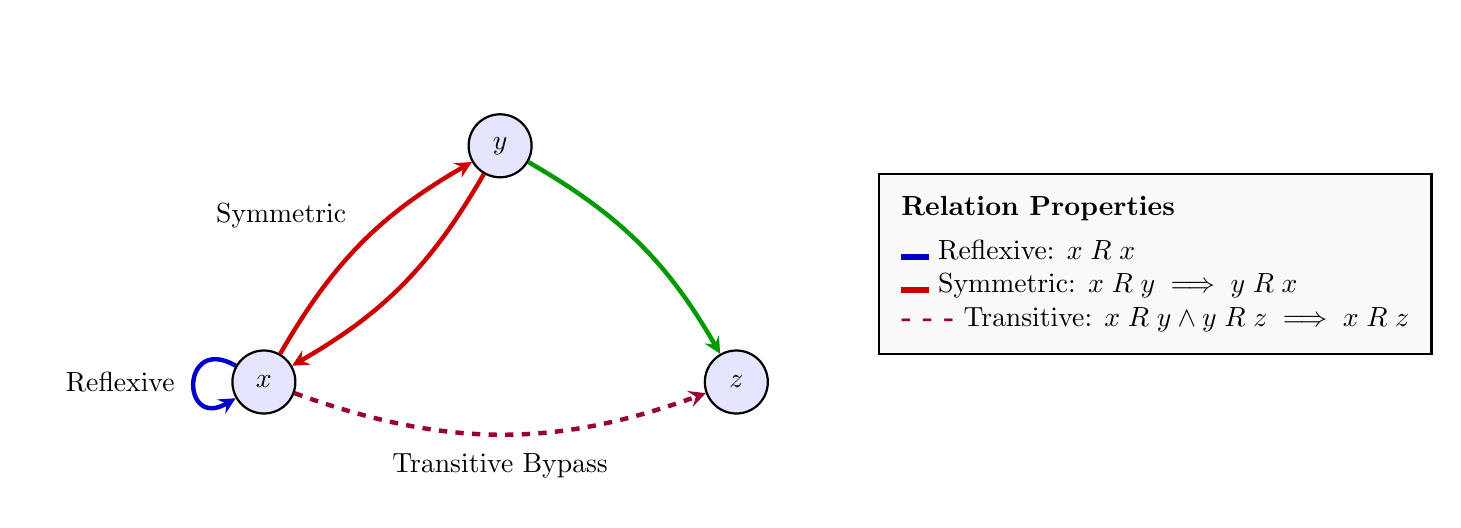
\begin{tikzpicture}[scale=1.5, >=stealth, node distance=2.5cm, thick]
    % Background layer for safety
    \fill[white] (-2,-1) rectangle (6, 3);

    % Nodes
    \node[circle, draw=black, fill=blue!10, minimum size=8mm] (X) at (0, 0) {$x$};
    \node[circle, draw=black, fill=blue!10, minimum size=8mm] (Y) at (2, 2) {$y$};
    \node[circle, draw=black, fill=blue!10, minimum size=8mm] (Z) at (4, 0) {$z$};

    % Reflexive Loop
    \draw[->, ultra thick, blue!80!black] (X) edge[loop left, out=150, in=210, looseness=5] node[left=3pt, text=black] {Reflexive} (X);

    % Symmetric Arrows
    \draw[->, ultra thick, red!80!black] (X) to[bend left=15] node[above left=2pt, text=black] {Symmetric} (Y);
    \draw[->, ultra thick, red!80!black] (Y) to[bend left=15] (X);

    % Transitive Chain
    \draw[->, ultra thick, green!60!black] (Y) to[bend left=15] (Z);
    \draw[->, ultra thick, purple!80!black, dashed] (X) to[bend right=20] node[below=3pt, text=black] {Transitive Bypass} (Z);

    % Legend using single-node multiline rule and anchor pivot
    \node[align=left, draw=black, fill=gray!5, inner sep=8pt, anchor=west] at (5.2, 1) {
        \textbf{Relation Properties}\\[4pt]
        \textcolor{blue!80!black}{\rule{10pt}{2pt}} Reflexive: $x \mathrel{R} x$ \\
        \textcolor{red!80!black}{\rule{10pt}{2pt}} Symmetric: $x \mathrel{R} y \implies y \mathrel{R} x$ \\
        \textcolor{purple!80!black}{\textbf{- - -}} Transitive: $x \mathrel{R} y \land y \mathrel{R} z \implies x \mathrel{R} z$
    };
\end{tikzpicture}
\end{center}

\subsection{Heuristics \& Pitfalls}
\begin{itemize}
    \item \textbf{The Vacuous Trap:} Never assume a relation is \textit{not} transitive just because it has very few elements. If you cannot find a specific trio $x, y, z$ that breaks the rule, the relation \textit{is} transitive.
    \item \textbf{Inverse vs. Reciprocal:} Do not confuse the inverse relation $R^{-1}$ with algebraic reciprocals. $R^{-1}$ swaps coordinates; it does not mean $1/R$.
    \item \textbf{The "All or Nothing" Fallacy:} A relation failing to be symmetric does \textit{not} mean it is antisymmetric. It simply means there is at least one one-way street.
\end{itemize}

\newpage

% ==========================================
% PART 5: CONCEPTUAL SYNTHESIS
% ==========================================
\section{Conceptual Synthesis and The "Big Picture"}

\subsection{A) Thematic Connections}
The central theme of this chapter is \textbf{structuring abstract spaces}. In basic set theory, a set is just an unstructured bag of elements. By defining a relation $R$ on a set, we impose a geometry or a topology onto that set. 
When a relation possesses all three properties (reflexive, symmetric, transitive), it becomes an \textit{Equivalence Relation}. This is a profound mathematical milestone because it allows us to treat distinct objects as if they were the same, provided they share a specific attribute. It formalizes the concept of "sameness" beyond strict equality.

\subsection{B) Forward and Backward Links}
\begin{itemize}
    \item \textbf{Backward Links:} This topic directly extends Cartesian products and basic predicate logic. The proofs rely heavily on the logical structure of implications ($P \implies Q$) established in introductory discrete math.
    \item \textbf{Forward Links:} Understanding relations is the absolute bedrock for advanced mathematics. 
    \begin{itemize}
        \item In \textbf{Abstract Algebra}, equivalence relations create \textit{Quotient Groups} and \textit{Cosets}.
        \item In \textbf{Measure Theory and Probability}, relations help define $\sigma$-algebras by partitioning sample spaces into measurable equivalence classes.
        \item In \textbf{Topology}, equivalence relations are used to glue spaces together (e.g., turning a flat plane into a torus by defining an equivalence relation on the edges).
    \end{itemize}
\end{itemize}

% ==========================================
% PART 6: ABSTRACT REAL-WORLD MODELING
% ==========================================
\section{Abstract Real-World Modeling (AI, ML, \& Quant Finance)}

\subsection{A) Concrete Scenarios}
\begin{enumerate}
    \item \textbf{Reinforcement Learning (State Space Reduction):} In Markov Decision Processes (MDPs), the state space can be astronomically large. AI researchers use an equivalence relation called \textit{Bisimulation} to group states that yield identical future reward distributions and transition probabilities. This compresses the state space, making the RL agent train exponentially faster.
    \item \textbf{Quantitative Finance (Arbitrage Equivalence):} In derivative pricing, two distinct portfolios are considered "equivalent" (an equivalence relation) if they yield the exact same payoff in all future states of the world. By the Law of One Price, equivalent portfolios must have the same current price, forming the basis of risk-neutral valuation.
\end{enumerate}

\subsection{B) Model Problem Setup: Bisimulation in Markov Decision Processes}
Let us rigorously model state equivalence in an AI environment. 
Define a Markov Decision Process as a tuple $\mathcal{M} = (S, A, P, R, \gamma)$, where $S$ is a finite state space, $A$ is the action space, $P(s' \mid s, a)$ is the transition probability measure, and $R(s, a)$ is the reward function.

We define a relation $E \subseteq S \times S$. We say two states are bisimilar, denoted $s_1 \mathrel{E} s_2$, if for all actions $a \in A$:
\begin{enumerate}
    \item $R(s_1, a) = R(s_2, a)$
    \item For every equivalence class $C \in S/E$ (the partition of $S$ generated by $E$), the transition probabilities to that class are identical:
    \[ \displaystyle \sum_{s' \in C} P(s' \mid s_1, a) = \sum_{s' \in C} P(s' \mid s_2, a) \]
\end{enumerate}
\textbf{Theoretical Goal:} Prove that $E$ is an equivalence relation (reflexive, symmetric, transitive). Once proven, the AI algorithm can operate on the quotient space $S/E$ rather than $S$. The Bellman optimality equation is then solved over the reduced space:
\[ \displaystyle V^*(C) = \max_{a \in A} \left( R(C, a) + \gamma \sum_{C' \in S/E} P(C' \mid C, a) V^*(C') \right) \]
This mathematical abstraction directly translates to massive computational savings in deep reinforcement learning architectures.

\newpage

% ==========================================
% PART 7: COMMON VARIATIONS
% ==========================================
\section{Common Variations and Untested Concepts}

A critical concept often taught alongside basic relations, but missing from the provided homework, is the \textbf{Closure of a Relation}.

\begin{definition}[Transitive Closure]
Let $R$ be a relation on a set $A$. The transitive closure of $R$, denoted $R^*$, is the smallest transitive relation on $A$ that contains $R$. It is mathematically defined as the intersection of all transitive relations containing $R$, or constructively as:
\[ \displaystyle (x, y) \in R^* \iff \exists \text{ a path } x = a_0, a_1, \dots, a_n = y \text{ such that } (a_i, a_{i+1}) \in R \text{ for all } i. \]
\end{definition}

\textbf{Worked Example:} Let $A = \{1, 2, 3, 4\}$ and $R = \{(1, 2), (2, 3), (3, 4)\}$. Find $R^*$.
\begin{proof}[Solution]
We must add all pairs that can be reached via intermediate steps.
\begin{itemize}
    \item Paths of length 1: $(1, 2), (2, 3), (3, 4)$
    \item Paths of length 2: Since $1 \to 2 \to 3$, we add $(1, 3)$. Since $2 \to 3 \to 4$, we add $(2, 4)$.
    \item Paths of length 3: Since $1 \to 2 \to 3 \to 4$, we add $(1, 4)$.
\end{itemize}
Thus, $R^* = \{(1, 2), (2, 3), (3, 4), (1, 3), (2, 4), (1, 4)\}$.
\end{proof}

% ==========================================
% PART 8: ADVANCED DIAGNOSTIC TESTING
% ==========================================
\section{Advanced Diagnostic Testing: "Find the Flaw"}

Below are five proofs related to relations. Each contains a subtle, critical logical flaw. Your task as a student is to find the error.

\textbf{Problem 1:} \textit{Claim: If a relation $R$ on a set $A$ is symmetric and transitive, then it must also be reflexive.}
\begin{proof}[Flawed Proof]
Let $x \in A$. We want to show $(x, x) \in R$. Since $R$ is symmetric, if $(x, y) \in R$, then $(y, x) \in R$. Since $R$ is transitive, we know that $(x, y) \in R$ and $(y, x) \in R$ implies $(x, x) \in R$. Therefore, $R$ is reflexive. $\blacksquare$
\end{proof}

\textbf{Problem 2:} \textit{Claim: The relation $R = \{(x, y) \in \R \times \R : x < y\}$ is transitive.}
\begin{proof}[Flawed Proof]
Assume $x \mathrel{R} y$ and $y \mathrel{R} z$. This means $x < y$ and $y < z$. Adding these inequalities gives $x + y < y + z$. Subtracting $y$ from both sides yields $x < z$. Thus $x \mathrel{R} z$. $\blacksquare$
\end{proof}

\textbf{Problem 3:} \textit{Claim: For any relation $R$ from $A$ to $B$, $\dom(R^{-1}) = \dom(R)$.}
\begin{proof}[Flawed Proof]
Let $x \in \dom(R^{-1})$. By definition, there exists $y$ such that $(x, y) \in R^{-1}$. By the definition of inverse, this means $(y, x) \in R$. Since $x$ is part of an ordered pair in $R$, $x$ must be in the domain of $R$. Thus $\dom(R^{-1}) \subseteq \dom(R)$. A similar argument shows the reverse inclusion. $\blacksquare$
\end{proof}

\textbf{Problem 4:} \textit{Claim: The relation $R = \emptyset$ on $A = \{1\}$ is an equivalence relation.}
\begin{proof}[Flawed Proof]
To be an equivalence relation, $R$ must be reflexive, symmetric, and transitive. 
Symmetry: If $(x, y) \in \emptyset$, then $(y, x) \in \emptyset$. This is vacuously true.
Transitivity: If $(x, y) \in \emptyset$ and $(y, z) \in \emptyset$, then $(x, z) \in \emptyset$. Vacuously true.
Reflexivity: For all $x \in A$, if $x \in \emptyset$, then $(x, x) \in \emptyset$. Vacuously true.
Thus, $R$ is an equivalence relation. $\blacksquare$
\end{proof}

\textbf{Problem 5:} \textit{Claim: If $R_1$ and $R_2$ are transitive relations on $A$, then $R_1 \cup R_2$ is transitive.}
\begin{proof}[Flawed Proof]
Assume $(x, y) \in R_1 \cup R_2$ and $(y, z) \in R_1 \cup R_2$. This means the pairs belong to either $R_1$ or $R_2$. Since both $R_1$ and $R_2$ are transitive, the chain from $x$ to $y$ to $z$ guarantees that $(x, z)$ is in the respective relation. Therefore, $(x, z) \in R_1 \cup R_2$. $\blacksquare$
\end{proof}

\vspace{2em}
\subsection*{Solution Key: Resolutions to the Flaws}
\begin{itemize}
    \item \textbf{Resolution 1:} The proof assumes there exists some $y \in A$ such that $(x, y) \in R$. If $x$ is completely isolated (related to nothing), the premise $(x, y) \in R$ is false, and we cannot deduce $(x, x) \in R$.
    \item \textbf{Resolution 2:} The algebraic manipulation is valid, but it is a circular justification. The property $x < y \land y < z \implies x < z$ is an axiom of the real numbers (the definition of order). Proving it by adding inequalities relies on the very order properties you are trying to establish.
    \item \textbf{Resolution 3:} The element $x$ in $(y, x) \in R$ is the \textit{second} coordinate. Therefore, $x \in \range(R)$, not $\dom(R)$. The correct statement is $\dom(R^{-1}) = \range(R)$.
    \item \textbf{Resolution 4:} The definition of reflexivity is $\forall x \in A, (x, x) \in R$. It is \textit{not} a conditional statement "if $x \in R$". Since $1 \in A$, we must have $(1, 1) \in R$. But $R = \emptyset$, so it fails reflexivity.
    \item \textbf{Resolution 5:} The flaw is assuming $(x, y)$ and $(y, z)$ belong to the \textit{same} relation. What if $(x, y) \in R_1$ and $(y, z) \in R_2$? Neither $R_1$ nor $R_2$ individually has the full chain, so neither is forced to contain $(x, z)$. (Counterexample: $R_1 = \{(1,2)\}$, $R_2 = \{(2,3)\}$. $R_1 \cup R_2$ is not transitive).
\end{itemize}

\end{document}